\documentclass[11pt]{report}
\usepackage[italian]{babel}
\usepackage[utf8]{inputenc}
\usepackage[T1]{fontenc}
\usepackage[nomarginpar]{geometry}
\usepackage{graphicx}
\graphicspath{ {images/} }

\usepackage[pdftex,
			pdfauthor={Eugenio Severi, Stefano Belli},
			pdftitle={Progetto ASW - id3king-js},
			pdfsubject={Relazione progetto Applicazioni e Servizi Web},
			pdfkeywords={id3king id3king-js ASW},
			pdfproducer={Latex with hyperref},
			pdfcreator={pdflatex}]{hyperref}
\pagestyle{plain}

\begin{document}
\title{Progetto di Applicazioni e Servizi Web\\id3king-js}
\author{Eugenio Severi, Stefano Belli}
\date{A.A. 2016-2017}
\begin{titlepage}
	\maketitle
\end{titlepage}

\setcounter{chapter}{1}
\section{Introduzione}
L'escursionismo è un attività motoria nel quale viene percorso un certo tragitto nel territorio su percorsi tipicamente agevoli, a scopo ricreativo o di studio.
\\Essendo un attività a basso sforzo fisico e molto modulabile nella sua difficoltà, è una pratica molto diffusa nel mondo e nel nostro paese da tutte le fasce d'età.\\ 
I percorsi solitamente utilizzati dagli escursionisti sono interamente mappati su apposite cartine topografiche, e il loro stato di percorrenza viene mantenuto costantemente da alcuni enti preposti come il C.A.I (Club Alpino Italiano).
\\Tuttavia, l'escursionismo è una pratica che richiede molta attenzione nella sua pianificazione, in quanto è facile sbagliare la stima della lunghezza del percorso o il suo dislivello. 
\\Molti escursionisti "occasionali" si ritrovano (loro malgrado) a capire esattamente le difficoltà di un percorso soltanto una volta sul luogo, magari a metà dell'escursione.
\\\\Fortunatamente, alcuni gruppi di escursionisti amatoriali redigono e pubblicano della documentazione sulle escursioni da loro intraprese: il più famoso di essi, perlomeno nella zona emiliano-romagnola, è \textit{id3king}.
\\Il sito del gruppo (www.id3king.it) infatti viene aggiornato periodicamente, con nuove escursioni inserite spesso settimanalmente; per ogni escursione presente, è possibile scaricarne il tracciato GPS, la tabella dei toponimi e una sezione della cartina del percorso, oltre a molte altre informazioni.
\\Data la relativa difficoltà di trovare informazioni così dettagliate sui percorsi escursionistici e di una tale entità (allo stato attuale, il sito presenta oltre 890 escursioni documentate su un arco di 18 anni!), è evidente che il lavoro di questo gruppo sia di enorme rilevanza per tutti gli appassionati di escursionismo.
\\Tuttavia, allo stato attuale il sito del gruppo non consente di filtrare a piacimento le escursioni inserite, così come ordinarle secondo un altro criterio oltre a quello della data di inserimento; queste mancanze rendono piuttosto difficoltoso trovare rapidamente l'escursione adatta alle proprie esigenze.
\\\\A causa di queste mancanze, è nato il progetto \textit{id3king-js}: ottenuto il consenso da parte degli amministratori del sito, infatti, si è deciso di progettare e sviluppare una web app che esegua lo scraping dell'originale e proponga i dati presenti in maniera maggiormente fruibile e funzionale, ad esempio permettendo una ricerca basata su parametri e la creazione di profili utente per memorizzare dati di interesse.
% TODO: diagramma dei casi d'uso
\pagebreak
\section{Architettura}
Come già anticipato nell'introduzione, l'applicazione dovrà consentire di filtrare e riordinare gli itinerari del sito per consentire una più veloce individuazione di un percorso in base a una certa esigenza.
\\Ad esempio, un utente alla ricerca di un percorso non troppo impegnativo potrebbe pensare di filtrare tutti gli itinerari con lunghezza e dislivello inferiori a un certo quantitativo, e magari posti nella zona del lago di Ridracoli (FC).
\\Comunque, le funzionalità offerte dall'applicazione possono essere riassunte con il seguente diagramma dei casi d'uso: 
\\
\begin{center}
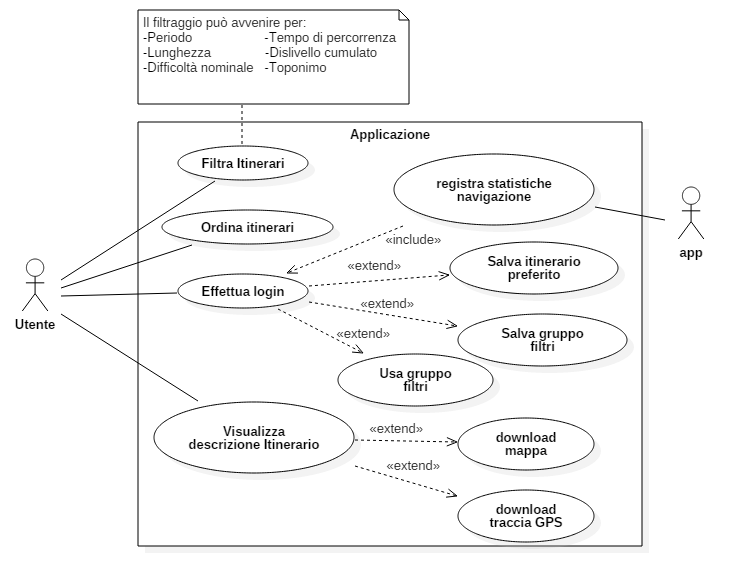
\includegraphics[scale=0.5]{use_case_diagram}
\end{center}
Per poter fornire all'utente tutte le funzionalità previste dal diagramma dei casi d'uso, è triviale la necessità di sviluppare un apposito server dedicato che possa gestire le sessioni utente e restituire gli itinerari presenti sul sito; pertanto, l'architettura del sistema è basata su una classica soluzione client-server.
\\Il server, inoltre, si occuperà di effettuare periodicamente lo scraping del sito: i dati estratti verranno riversati in un apposito database relazionale da cui si potrà attingere per ogni richiesta degli utenti.\\
\\
Riepilogando, trattandosi di un'applicazione di tipo client-server, l'architettura sarà composta dai seguenti componenti:
\begin{itemize}
	\item un insieme di client che effettuano richieste al servizio;
	\item un server web che risponde alle esigenze dei client;
	\item un database relazionale per l'archiviazione dei dati.
\end{itemize}
Opzionalmente è possibile rendere l'applicazione scalabile orizzontalmente e resistente ai guasti tramite più server web e load balancer.
\\Analogamente, è possibile utilizzare non un singolo DBMS, ma una configurazione cluster.
\\Ai fini di questo progetto si è scelto di utilizzare un unico server cloud di tipo \textit{IaaS} (Infrastructure as a Service), fornito da un provider, sul quale saranno installati tutti i servizi necessari al funzionamento dell'applicazione.
\\In base ai requisiti precedentemente definiti, come framework di sviluppo si è valutato di usare \textit{Node.js}, che prevede l'utilizzo di tecnologie web sia client-side che server-side e consente di utilizzare un modello di comunicazione event-driven, particolarmente utile in un'applicazione di rete.
Saranno presenti interfacce REST, che prevedono una comunicazione \textit{stateless} (ovvero non necessita della memorizzazione di alcun contesto client sul server), consentono di implementare facilmente un'architettura scalabile a livelli con nodi di commutazione intermedi e sono universalmente riconosciute e supportate, essendo basate tu HTTP+TCP+IP.
% TODO: diagramma di deployment

\section{Sicurezza}
Data la natura di rete dell'applicazione e poiché verranno trattati anche alcuni dati personali degli utenti, è opportuno considerare la sicurezza già in fase di progettazione, onde evitare lacune successive difficili da individuare e rimuovere:
\begin{itemize}
	\item tutte le comunicazioni di rete devono essere crittografate e autenticate con SSL/TLS per prevenire intercettazioni e attacchi \textit{man-in-the-middle};
	\item tutti gli input degli utenti devono essere validati per impedire lo sfruttamento di \textit{SQL injection} e \textit{buffer overflow}.
\end{itemize}
Le credenziali degli utenti dovranno inoltre essere memorizzate sotto forma di hash della password e con \textit{salt}, onde rendere difficoltoso per un attaccante decifrare le password.
A tale scopo si è scelta la funzione \textit{bcrypt}.

\section{Back-end}
Verrà ora descritto il funzionamento del back-end.
%TODO: diagramma delle classi e/o di sequenza
%TODO: Dati e database, controller (pattern MVC), interazioni con il db, scraper.

\section{Front-end}
%TODO: Angular in generale, pattern MVC (e altri?), descrizione interfaccia grafica (spiegazione funzioni principali con qualche screenshot).

\section{Conclusioni}


\end{document}
\endinput